\documentclass[border=1pt]{standalone}
\usepackage{pgfplots}
\usepgfplotslibrary{groupplots,fillbetween}
\usepackage{animate}

\usepackage{pgf}
\usepackage{tikz}

\usetikzlibrary{fit}
\usetikzlibrary{positioning}
\usetikzlibrary{arrows}
\usetikzlibrary{automata}
\usetikzlibrary{backgrounds}
\usetikzlibrary{shapes.misc}

% https://tex.stackexchange.com/questions/118223/drawing-little-semicircle-to-show-that-two-intersecting-lines-are-not-connected
\usetikzlibrary{calc}

% \intersect{<p1>}{<p2>}{<q1>}{<q2>}
% draws the line p1--p2, showing a little semicircle
% where it intersects the line q1--q2.
\newcommand\intersect[4]{
  \draw let \p{c} = (intersection of #1--#2 and #3--#4) in
    (#1) -- ($(\p{c})!0.75mm!(#1)$) 
    to[bend right=90] ($(\p{c})!0.75mm!(#2)$) -- (#2)
}


\begin{document}    

  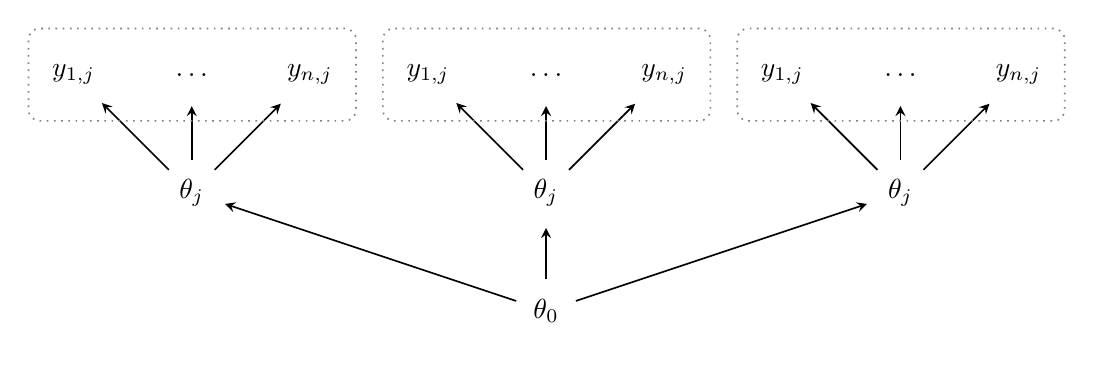
\begin{tikzpicture}[
            > = stealth, % arrow head style
            shorten > = 1pt, % don't touch arrow head to node
            auto,
            node distance = 1.5cm, % distance between nodes
            semithick % line style
        ]

        \tikzstyle{every state}=[
            draw = none,
            thick,
            fill = white,
            minimum size = 4mm
        ]F
% data level
        \node[state] (Y1) [] {$y_{1,j}$};
           \node[state] (Y2) [right of = Y1] {$\dots$};
            \node[state] (Y3) [right of = Y2] {$y_{n,j}$};
 
        \node[state] (Y1B) [right of = Y3] {$y_{1,j}$};
           \node[state] (Y2B) [right of = Y1B] {$\dots$};
            \node[state] (Y3B) [right of = Y2B] {$y_{n,j}$};
            
        \node[state] (Y1C) [right of = Y3B] {$y_{1,j}$};
           \node[state] (Y2C) [right of = Y1C] {$\dots$};
            \node[state] (Y3C) [right of = Y2C] {$y_{n,j}$};            
            
       \node[state] (YR1) [below of = Y2] {$\theta_j$};
       \node[state] (YR2) [below of = Y2B] {$\theta_j$};
       \node[state] (YR3) [below of = Y2C] {$\theta_j$};
      
        \path[->] (YR1) edge node {} (Y1);      
        \path[->] (YR1) edge node {} (Y2);
        \path[->] (YR1) edge node {} (Y3);

        \path[->] (YR2) edge node {} (Y1B);
        \path[->] (YR2) edge node {} (Y2B);
        \path[->] (YR2) edge node {} (Y3B);

        \path[->] (YR3) edge node {} (Y1C);
        \path[->] (YR3) edge node {} (Y2C);
        \path[->] (YR3) edge node {} (Y3C);
                                    
       \node[state] (GLOBAL) [below of = YR2] {$\theta_0$};
       
        \path[->] (GLOBAL) edge node {} (YR1);
        \path[->] (GLOBAL) edge node {} (YR2);
        \path[->] (GLOBAL) edge node {} (YR3);        
                  
    \begin{scope}[draw=gray]
   \node [draw,dotted,fit=(Y1) (Y3) , rounded corners, inner sep=.1cm] {};
   \node [draw,dotted,fit=(Y1B) (Y3B) ,  rounded corners, inner sep=.1cm] {};
   \node [draw,dotted,fit=(Y1C) (Y3C) , rounded corners, inner sep=.1cm] {};
  \end{scope}
  
  \end{tikzpicture}
  
  \end{document}